
%% bare_conf.tex
%% V1.3
%% 2007/01/11
%% by Michael Shell
%% See:
%% http://www.michaelshell.org/
%% for current contact information.
%%
%% This is a skeleton file demonstrating the use of IEEEtran.cls
%% (requires IEEEtran.cls version 1.7 or later) with an IEEE conference paper.
%%
%% Support sites:
%% http://www.michaelshell.org/tex/ieeetran/
%% http://www.ctan.org/tex-archive/macros/latex/contrib/IEEEtran/
%% and
%% http://www.ieee.org/

%%*************************************************************************
%% Legal Notice:
%% This code is offered as-is without any warranty either expressed or
%% implied; without even the implied warranty of MERCHANTABILITY or
%% FITNESS FOR A PARTICULAR PURPOSE! 
%% User assumes all risk.
%% In no event shall IEEE or any contributor to this code be liable for
%% any damages or losses, including, but not limited to, incidental,
%% consequential, or any other damages, resulting from the use or misuse
%% of any information contained here.
%%
%% All comments are the opinions of their respective authors and are not
%% necessarily endorsed by the IEEE.
%%
%% This work is distributed under the LaTeX Project Public License (LPPL)
%% ( http://www.latex-project.org/ ) version 1.3, and may be freely used,
%% distributed and modified. A copy of the LPPL, version 1.3, is included
%% in the base LaTeX documentation of all distributions of LaTeX released
%% 2003/12/01 or later.
%% Retain all contribution notices and credits.
%% ** Modified files should be clearly indicated as such, including  **
%% ** renaming them and changing author support contact information. **
%%
%% File list of work: IEEEtran.cls, IEEEtran_HOWTO.pdf, bare_adv.tex,
%%                    bare_conf.tex, bare_jrnl.tex, bare_jrnl_compsoc.tex
%%*************************************************************************

% *** Authors should verify (and, if needed, correct) their LaTeX system  ***
% *** with the testflow diagnostic prior to trusting their LaTeX platform ***
% *** with production work. IEEE's font choices can trigger bugs that do  ***
% *** not appear when using other class files.                            ***
% The testflow support page is at:
% http://www.michaelshell.org/tex/testflow/



% Note that the a4paper option is mainly intended so that authors in
% countries using A4 can easily print to A4 and see how their papers will
% look in print - the typesetting of the document will not typically be
% affected with changes in paper size (but the bottom and side margins will).
% Use the testflow package mentioned above to verify correct handling of
% both paper sizes by the user's LaTeX system.
%
% Also note that the "draftcls" or "draftclsnofoot", not "draft", option
% should be used if it is desired that the figures are to be displayed in
% draft mode.
%
\documentclass[10pt, conference, compsocconf]{IEEEtran}
% Add the compsocconf option for Computer Society conferences.
%
% If IEEEtran.cls has not been installed into the LaTeX system files,
% manually specify the path to it like:
% \documentclass[conference]{../sty/IEEEtran}





% Some very useful LaTeX packages include:
% (uncomment the ones you want to load)


% *** MISC UTILITY PACKAGES ***
%
%\usepackage{ifpdf}
% Heiko Oberdiek's ifpdf.sty is very useful if you need conditional
% compilation based on whether the output is pdf or dvi.
% usage:
% \ifpdf
%   % pdf code
% \else
%   % dvi code
% \fi
% The latest version of ifpdf.sty can be obtained from:
% http://www.ctan.org/tex-archive/macros/latex/contrib/oberdiek/
% Also, note that IEEEtran.cls V1.7 and later provides a builtin
% \ifCLASSINFOpdf conditional that works the same way.
% When switching from latex to pdflatex and vice-versa, the compiler may
% have to be run twice to clear warning/error messages.






% *** CITATION PACKAGES ***
%
%\usepackage{cite}
% cite.sty was written by Donald Arseneau
% V1.6 and later of IEEEtran pre-defines the format of the cite.sty package
% \cite{} output to follow that of IEEE. Loading the cite package will
% result in citation numbers being automatically sorted and properly
% "compressed/ranged". e.g., [1], [9], [2], [7], [5], [6] without using
% cite.sty will become [1], [2], [5]--[7], [9] using cite.sty. cite.sty's
% \cite will automatically add leading space, if needed. Use cite.sty's
% noadjust option (cite.sty V3.8 and later) if you want to turn this off.
% cite.sty is already installed on most LaTeX systems. Be sure and use
% version 4.0 (2003-05-27) and later if using hyperref.sty. cite.sty does
% not currently provide for hyperlinked citations.
% The latest version can be obtained at:
% http://www.ctan.org/tex-archive/macros/latex/contrib/cite/
% The documentation is contained in the cite.sty file itself.






% *** GRAPHICS RELATED PACKAGES ***
%
\ifCLASSINFOpdf
  \usepackage[pdftex]{graphicx}
  % declare the path(s) where your graphic files are
  % \graphicspath{{../pdf/}{../jpeg/}}
  % and their extensions so you won't have to specify these with
  % every instance of \includegraphics
  % \DeclareGraphicsExtensions{.pdf,.jpeg,.png}
\else
  % or other class option (dvipsone, dvipdf, if not using dvips). graphicx
  % will default to the driver specified in the system graphics.cfg if no
  % driver is specified.
  \usepackage[dvips]{graphicx}
  % declare the path(s) where your graphic files are
  % \graphicspath{{../eps/}}
  % and their extensions so you won't have to specify these with
  % every instance of \includegraphics
  % \DeclareGraphicsExtensions{.eps}
\fi

% graphicx was written by David Carlisle and Sebastian Rahtz. It is
% required if you want graphics, photos, etc. graphicx.sty is already
% installed on most LaTeX systems. The latest version and documentation can
% be obtained at: 
% http://www.ctan.org/tex-archive/macros/latex/required/graphics/
% Another good source of documentation is "Using Imported Graphics in
% LaTeX2e" by Keith Reckdahl which can be found as epslatex.ps or
% epslatex.pdf at: http://www.ctan.org/tex-archive/info/
%
% latex, and pdflatex in dvi mode, support graphics in encapsulated
% postscript (.eps) format. pdflatex in pdf mode supports graphics
% in .pdf, .jpeg, .png and .mps (metapost) formats. Users should ensure
% that all non-photo figures use a vector format (.eps, .pdf, .mps) and
% not a bitmapped formats (.jpeg, .png). IEEE frowns on bitmapped formats
% which can result in "jaggedy"/blurry rendering of lines and letters as
% well as large increases in file sizes.
%
% You can find documentation about the pdfTeX application at:
% http://www.tug.org/applications/pdftex





% *** MATH PACKAGES ***
%
\usepackage[cmex10]{amsmath}
% A popular package from the American Mathematical Society that provides
% many useful and powerful commands for dealing with mathematics. If using
% it, be sure to load this package with the cmex10 option to ensure that
% only type 1 fonts will utilized at all point sizes. Without this option,
% it is possible that some math symbols, particularly those within
% footnotes, will be rendered in bitmap form which will result in a
% document that can not be IEEE Xplore compliant!
%
% Also, note that the amsmath package sets \interdisplaylinepenalty to 10000
% thus preventing page breaks from occurring within multiline equations. Use:
%\interdisplaylinepenalty=2500
% after loading amsmath to restore such page breaks as IEEEtran.cls normally
% does. amsmath.sty is already installed on most LaTeX systems. The latest
% version and documentation can be obtained at:
% http://www.ctan.org/tex-archive/macros/latex/required/amslatex/math/





% *** SPECIALIZED LIST PACKAGES ***
%
%\usepackage{algorithmic}
% algorithmic.sty was written by Peter Williams and Rogerio Brito.
% This package provides an algorithmic environment fo describing algorithms.
% You can use the algorithmic environment in-text or within a figure
% environment to provide for a floating algorithm. Do NOT use the algorithm
% floating environment provided by algorithm.sty (by the same authors) or
% algorithm2e.sty (by Christophe Fiorio) as IEEE does not use dedicated
% algorithm float types and packages that provide these will not provide
% correct IEEE style captions. The latest version and documentation of
% algorithmic.sty can be obtained at:
% http://www.ctan.org/tex-archive/macros/latex/contrib/algorithms/
% There is also a support site at:
% http://algorithms.berlios.de/index.html
% Also of interest may be the (relatively newer and more customizable)
% algorithmicx.sty package by Szasz Janos:
% http://www.ctan.org/tex-archive/macros/latex/contrib/algorithmicx/




% *** ALIGNMENT PACKAGES ***
%
%\usepackage{array}
% Frank Mittelbach's and David Carlisle's array.sty patches and improves
% the standard LaTeX2e array and tabular environments to provide better
% appearance and additional user controls. As the default LaTeX2e table
% generation code is lacking to the point of almost being broken with
% respect to the quality of the end results, all users are strongly
% advised to use an enhanced (at the very least that provided by array.sty)
% set of table tools. array.sty is already installed on most systems. The
% latest version and documentation can be obtained at:
% http://www.ctan.org/tex-archive/macros/latex/required/tools/


%\usepackage{mdwmath}
%\usepackage{mdwtab}
% Also highly recommended is Mark Wooding's extremely powerful MDW tools,
% especially mdwmath.sty and mdwtab.sty which are used to format equations
% and tables, respectively. The MDWtools set is already installed on most
% LaTeX systems. The lastest version and documentation is available at:
% http://www.ctan.org/tex-archive/macros/latex/contrib/mdwtools/


% IEEEtran contains the IEEEeqnarray family of commands that can be used to
% generate multiline equations as well as matrices, tables, etc., of high
% quality.


%\usepackage{eqparbox}
% Also of notable interest is Scott Pakin's eqparbox package for creating
% (automatically sized) equal width boxes - aka "natural width parboxes".
% Available at:
% http://www.ctan.org/tex-archive/macros/latex/contrib/eqparbox/





% *** SUBFIGURE PACKAGES ***
%\usepackage[tight,footnotesize]{subfigure}
% subfigure.sty was written by Steven Douglas Cochran. This package makes it
% easy to put subfigures in your figures. e.g., "Figure 1a and 1b". For IEEE
% work, it is a good idea to load it with the tight package option to reduce
% the amount of white space around the subfigures. subfigure.sty is already
% installed on most LaTeX systems. The latest version and documentation can
% be obtained at:
% http://www.ctan.org/tex-archive/obsolete/macros/latex/contrib/subfigure/
% subfigure.sty has been superceeded by subfig.sty.



%\usepackage[caption=false]{caption}
%\usepackage[font=footnotesize]{subfig}
% subfig.sty, also written by Steven Douglas Cochran, is the modern
% replacement for subfigure.sty. However, subfig.sty requires and
% automatically loads Axel Sommerfeldt's caption.sty which will override
% IEEEtran.cls handling of captions and this will result in nonIEEE style
% figure/table captions. To prevent this problem, be sure and preload
% caption.sty with its "caption=false" package option. This is will preserve
% IEEEtran.cls handing of captions. Version 1.3 (2005/06/28) and later 
% (recommended due to many improvements over 1.2) of subfig.sty supports
% the caption=false option directly:
%\usepackage[caption=false,font=footnotesize]{subfig}
%
% The latest version and documentation can be obtained at:
% http://www.ctan.org/tex-archive/macros/latex/contrib/subfig/
% The latest version and documentation of caption.sty can be obtained at:
% http://www.ctan.org/tex-archive/macros/latex/contrib/caption/




% *** FLOAT PACKAGES ***
%
%\usepackage{fixltx2e}
% fixltx2e, the successor to the earlier fix2col.sty, was written by
% Frank Mittelbach and David Carlisle. This package corrects a few problems
% in the LaTeX2e kernel, the most notable of which is that in current
% LaTeX2e releases, the ordering of single and double column floats is not
% guaranteed to be preserved. Thus, an unpatched LaTeX2e can allow a
% single column figure to be placed prior to an earlier double column
% figure. The latest version and documentation can be found at:
% http://www.ctan.org/tex-archive/macros/latex/base/



%\usepackage{stfloats}
% stfloats.sty was written by Sigitas Tolusis. This package gives LaTeX2e
% the ability to do double column floats at the bottom of the page as well
% as the top. (e.g., "\begin{figure*}[!b]" is not normally possible in
% LaTeX2e). It also provides a command:
%\fnbelowfloat
% to enable the placement of footnotes below bottom floats (the standard
% LaTeX2e kernel puts them above bottom floats). This is an invasive package
% which rewrites many portions of the LaTeX2e float routines. It may not work
% with other packages that modify the LaTeX2e float routines. The latest
% version and documentation can be obtained at:
% http://www.ctan.org/tex-archive/macros/latex/contrib/sttools/
% Documentation is contained in the stfloats.sty comments as well as in the
% presfull.pdf file. Do not use the stfloats baselinefloat ability as IEEE
% does not allow \baselineskip to stretch. Authors submitting work to the
% IEEE should note that IEEE rarely uses double column equations and
% that authors should try to avoid such use. Do not be tempted to use the
% cuted.sty or midfloat.sty packages (also by Sigitas Tolusis) as IEEE does
% not format its papers in such ways.





% *** PDF, URL AND HYPERLINK PACKAGES ***
%
%\usepackage{url}
% url.sty was written by Donald Arseneau. It provides better support for
% handling and breaking URLs. url.sty is already installed on most LaTeX
% systems. The latest version can be obtained at:
% http://www.ctan.org/tex-archive/macros/latex/contrib/misc/
% Read the url.sty source comments for usage information. Basically,
% \url{my_url_here}.


\usepackage{amssymb}
\usepackage{amsthm}

\theoremstyle{plain}
\newtheorem{thm}{Theorem} % reset theorem numbering for each chapter

\theoremstyle{definition}
\newtheorem{defn}[thm]{Definition} % definition numbers are dependent on theorem numbers
\newtheorem{exmp}[thm]{Example} % same for example numbers
% *** Do not adjust lengths that control margins, column widths, etc. ***
% *** Do not use packages that alter fonts (such as pslatex).         ***
% There should be no need to do such things with IEEEtran.cls V1.6 and later.
% (Unless specifically asked to do so by the journal or conference you plan
% to submit to, of course. )


% correct bad hyphenation here
\hyphenation{op-tical net-works semi-conduc-tor}


\begin{document}
%
% paper title
% can use linebreaks \\ within to get better formatting as desired
\title{Efficient Coalition Formation for Web Services}


% author names and affiliations
% use a multiple column layout for up to two different
% affiliations

\author{\IEEEauthorblockN{Ehsan Khosrowshahi Asl, Jamal Bentahar}
\IEEEauthorblockA{Faculty of Engineeing and Computer Science\\
Concordia University\\
Montreal, Canada\\
e\_khosr@encs.concordia.ca, bentahar@ciise.concordia.ca}
\and
\IEEEauthorblockN{Hadi Otrok, Rabeb Mizouni}
\IEEEauthorblockA{Department of Electrical and Computer Engineering\\
Khalifa University\\
Dubai, UAE\\
hadi.otrak, rabeb.mizouni@kustar:ac:ae}
}

% conference papers do not typically use \thanks and this command
% is locked out in conference mode. If really needed, such as for
% the acknowledgment of grants, issue a \IEEEoverridecommandlockouts
% after \documentclass

% for over three affiliations, or if they all won't fit within the width
% of the page, use this alternative format:
% 
%\author{\IEEEauthorblockN{Michael Shell\IEEEauthorrefmark{1},
%Homer Simpson\IEEEauthorrefmark{2},
%James Kirk\IEEEauthorrefmark{3}, 
%Montgomery Scott\IEEEauthorrefmark{3} and
%Eldon Tyrell\IEEEauthorrefmark{4}}
%\IEEEauthorblockA{\IEEEauthorrefmark{1}School of Electrical and Computer Engineering\\
%Georgia Institute of Technology,
%Atlanta, Georgia 30332--0250\\ Email: see http://www.michaelshell.org/contact.html}
%\IEEEauthorblockA{\IEEEauthorrefmark{2}Twentieth Century Fox, Springfield, USA\\
%Email: homer@thesimpsons.com}
%\IEEEauthorblockA{\IEEEauthorrefmark{3}Starfleet Academy, San Francisco, California 96678-2391\\
%Telephone: (800) 555--1212, Fax: (888) 555--1212}
%\IEEEauthorblockA{\IEEEauthorrefmark{4}Tyrell Inc., 123 Replicant Street, Los Angeles, California 90210--4321}}




% use for special paper notices
%\IEEEspecialpapernotice{(Invited Paper)}




% make the title area
\maketitle


\begin{abstract}

Web services are loosely-coupled business applications and willing to cooperate in distributed settings within different groups called communities. Communities aim to provide better efficiency, market share and total payoff. There are a number of proposed mechanisms and models on aggregating web services, however forming optimal and stable coalitions to maximize individual and community efficiency and income has got less attention. In this paper, we propose an efficient coalition formation mechanism using cooperative game-theoretic methods. We propose a mechanism for membership requests and selection of web services in the scenarios in which there are already established communities. Moreover, we analyze the scenarios in which we do not have pre-defined communities and we develop a mechanism for web services to form stable groups allowing them to maximize their efficiency and generate near-optimal (welfare-maximizing) communities. The theoretical and simulation results show that our algorithms provide web services and community owners with applicable and near-optimal decision making mechanisms.

\end{abstract}

\begin{IEEEkeywords}
Web services; Cooperative game thoery; Community of services;

\end{IEEEkeywords}


% For peer review papers, you can put extra information on the cover
% page as needed:
% \ifCLASSOPTIONpeerreview
% \begin{center} \bfseries EDICS Category: 3-BBND \end{center}
% \fi
%
% For peerreview papers, this IEEEtran command inserts a page break and
% creates the second title. It will be ignored for other modes.
\IEEEpeerreviewmaketitle

\section{Introduction}

Over the past years, web applications have become part of critical buisiness services. The increasing reliance on web-based applications has had significant implications for service providers and its users.

TODO on functional and non-functional requirements specially for critial applications \\

TODO on community of web services \\

TODO Problems of \cite{Chun02user-centricperformance, mcknight00a, DBLP:journals/internet/BenatallahSD03, Khosravifar:2009:AIR:1586636.1586906, Rosario:2008:PQS:1512146.1512290} \\

TODO Problems of \cite {DBLP:conf/IEEEscc/LimTMB12} having to cop and optimizing for with all weak web services reduces the optimal result\\

TODO Problems of \cite {DBLP:conf/IEEEscc/KhosravifarABT11} not considering the current web services in coalition and startegies are only based on master web service and new web service gain\\



%Some random text:
%A Web service is an interface that describes a collection of operations that are network-accessible through standardized XML messaging. A Web service performs a specific task or a set of tasks.A Web service is described using a standard, formal XML notation, called its service description, that provides all of the details necessary to interact with the service, including message formats (that detail the operations), transport protocols, and location. Web service descriptions are expressed in WSDL.
%
%Web services can become untrustworthy for four reasons: unfulfilled requirements,malicious acts and code changes, erratic Internet behaviors or resource scarcity that result in unacceptable delays, and the poor interoperation of selected services.
%
%A Web service is an independent service component that aims to serve a variety of needs; it is not a single specific application. When the selected Web service component does not thoroughly fulfill its target need, the service becomes untrustworthy. Testing a service to determine that it fulfills all requirements is tricky because testing must verify the satisfaction of both functional and nonfunctional requirements. The nonfunctional requirements (reliability, availability, survivability, interoperability, and a host of other attributes) decide the service quality and require individual testing. Because the user can invoke a Web service only over the Internet, the challenge is how to test for all possible use scenarios.How can testing determine that the service operates effectively and efficiently for a specific application and environment?

\section{Preliminaries}

In this section we discuss the parameters and preliminary concepts that we use in the rest of paper. The way communities of web services are structured and engineered is described thoroughly in \cite{DBLP:journals/ijebr/MaamarSTBB09}. 

\subsection{The Architecture and Entities }
\subsubsection{Web Services}
\subsubsection{Master Web Service of Communities}
\subsubsection{Users}

\subsection{Task Parameters}
\subsubsection{Request rate}
\subsubsection{Consumption}
\subsubsection{Requested Reponse Time}
\subsubsection{Requested Availability}
\subsubsection{Requested Success Rate}

\subsection{Web Sercive Parameters}
\subsubsection{Throughput}
\subsubsection{Capacity}
\subsubsection{Cost}
\subsubsection{Reponse Time}
\subsubsection{Availability}
\subsubsection{Reliability}
\subsubsection{Success Rate}
\subsubsection{Reputation}


\subsection{Cooperative Game Concepts}
Cooperative game is a branch of game theory that studies strategies of self-interested agents in a setting where agents can increase their payoff by binding agreements and cooperating in groups. We let N to be a set of players. Any subset S of N can form a group that we call it a $coalition$. A $coalitional game$ is a pair $G = (N, v)$ where v is $characteristic function$ which given a coalition is a function $v: 2^N \to \mathbb{R}$ which maps the set of agents of the coalition to a real number v(S), the worth of S. This number usually resembles the output or payoff or performance of these agents working together as a coalition.  If a coalition S forms then it can divide its worth, v(S) in any possible among its members. The payoff vector $x \in \mathbb{R}^S$ is the amount of payoff being distributed among agents of coalition S. The payoff vector satisfies two conditions:

\begin{itemize}
	\item $x \geq 0$ for all $i \in N$, and
	\item $\sum_{i \in S} x_i \leq v(S)$
\end{itemize}

The second condition is $feasibility$, according to equation below the payoff for each agent cannot be more than coalitions total gain. A payoff vector is also $efficient$ if all the payoff obtained by a coalition is distributed amongst coalition members: $\sum_{i \in S} x_i = v(S)$. This definition of characteristic function works in $transferable utility$ (TU) settings, where utility (payoff) is transferable from one player to other, in other words players have common currency and a unit of income is worth same for all players \cite{myerson1991game}.

When dealing with cooperative games, two issues need to get addressed: 1. What coalition to form (Canonical games)? 2. How to reward each member when a task is completed (Coalition-formation games)?

\subsubsection{Shapley value}

{\bf Definition 1 (Shapley value)} Given a cooperative game (N, v), the Shapley value of player i is given by\cite{shapley_value}: 
\begin{equation}\label{eq:shapley}
\sum_{S \subset N \backslash \left\{i\right\} } \frac{|S|! (n-|S|-1)!}{n!} (v(S \cup \left\{i\right\}) - v(S))
\end{equation}

Shapley value is a unique and fair solution concept for payoff distribution between agents. It basically rewards agents with amount of marginal contribution they have to the coalition.

\subsubsection{Core}

{\bf Definition 2 (Core)} A payoff vector x denoted by C(N,v) is in the core of a coalitional game (N, v) if and only if
\begin{equation}\label{eq:core}
\forall S \subseteq N, \sum_{x_i \in S} x_i \geq v(S)
\end{equation}
The core if is not empty is basically a set of payoff vectors (x) where no subset of players $S^\prime$ could gain more by deviating and making their own coalition $\sum_{i \in S^\prime} x_i \geq v(S^\prime)$. The sum of payoffs to the agents in any sub-coalition S is at least as large as the amount that these agents could earn by forming a coalition on their own. In a sense it is analogue to Nash equilibrium, except that it about deviations by groups of agents. The core is the strongest and most popular solution concept in cooperative game theory, however its computationally very heavy and is not computationally tractable as number of players increase. The core of some real-world problem games may be empty, which means having characteristic function $v$ there might be no possible distribution of payoff assuring stability of subgroups.

{\bf Definition 3 (Convex cooperative games)} A game with characteristic function v(S) is convex if:
\begin{equation}\label{eq:convex}
V(S) + V(T) \leq v(S \cup T) + v (S \cap T), \forall S,T \subseteq N.
\end{equation}

According to a classic result by Shapley \cite{S1971cores} convex games always have a non-empty core. We will use a variation of convexity condition in our algorithm to check whether our coalitions are stable.

\subsubsection{$\epsilon-Core$}\label{s:epsilon}
If core set is not empty, it means no coalition of players can gain anything by deviating, it is the strongest stable condition. An outcome would be unstable if a coalition can benefit even by a small amount from deviating. This is a strong requirement. In some situations, deviations can be costly or agents may have some loyalty to their coalitions or even it can be computationally intractable to find those small benefits. It would only make sense for a coalition to deviate if the gain from a deviation exceeded a particular cost for example the costs of deviation. $\epsilon-Core$ relaxes the notion of the core, and only require that no coalition can benefit significantly or within a constant amount($\epsilon$) by deviating.

\begin{equation}\label{eq:core}
\forall S \subseteq N, \sum_{x_i \in S} x_i \geq v(S) - \epsilon
\end{equation}

\subsubsection{Coalition Structure Formation}\label{sec:coalition}

Coalition structure formation is the problem of finding best partition of agents into teams, focusing more on optimizing the coalition's ``owner'' payoff. In these settings performance of individual agent is less important than the \emph{social welfare} of the system, which is the sum of the values of all teams. Having characteristic function game G, a coalition structure (CS) is \emph{socially optimal} is CS belongs to set $argmax_{CS \in CS_N}v(CS)$ where v(CS) is sum of the total valuation function of all coalitions inside CS $(v(CS) = \sum_{C \in CS_N}v(CS))$. The outcome of a characteristic function game in coalition structure settings, consists of two parts; first a disjoint partition of players (agents) into coalitions, called a \emph{coalition structure} (CS) and second a \emph{payoff vector} as mentioned in cooperative game solution concepts, which distributes the value of each coalition among its members.

\section{Problem Formulation and Modeling}

In this section, we present the architecture of different web service community models and formulate how both web services and community masters as rational agents would maximise their payoff.

\subsection {Web Services and A Grand Community}

In this scenario, there are is a community controller by its master web service. The community master has some request rate $(R_{master})$ from users. Web services need to join a community to be able to get tasks from a master web service. Each web service comes with different quality of service parameters and a throughput $(T_{ws})$. Throughput is the average rate of tasks a web service can perform. Therefore, the master web service is providing tasks with rate of $R_{ws}$ and web services perform tasks with some QoS output metrics and a rate or $T_{ws}$. 
In this setting, we define the value of the coalition as follows:
\begin{equation*}
output(C) = \sum_{ws}{(T_{ws} \times QoS_{ws})}
\end{equation*}

\begin{equation*}
v(C) = \left\{ 
  \begin{array}{l l}
    output(C) & \quad \text{if $\sum_{ws}{T_{ws}} \leq R_{master}$}\\
    output(C) \times \frac{R_{master}}{\sum_{ws}{T_{ws}}} & \quad \text{if $\sum_{ws}{T_{ws}} > R_{master}$}
  \end{array} \right.
\end{equation*}  

The output of a coalition of web services is the rate and quality of task they can perform. If the rate is more than master's input task rate, it means the web services inside the community are capable of doing more tasks than exists. Considering this the valuation function will balance the output performance and will be the exact amount and quality of work they can perform within the particular community. %** In the case where the limited tasks are distributed among web services uniformly, the value of coalition would be the proportion of the average QoS times their throughput to rate of available requests. **

In the first scenario, we only consider one grand coalition and analyse the system from point of view of one single master web service and a collection of web services. The master web service decides which members can join %or should leave% 
the community and distributes the income or tasks among its community members.

\begin{figure}[!t]
\centering
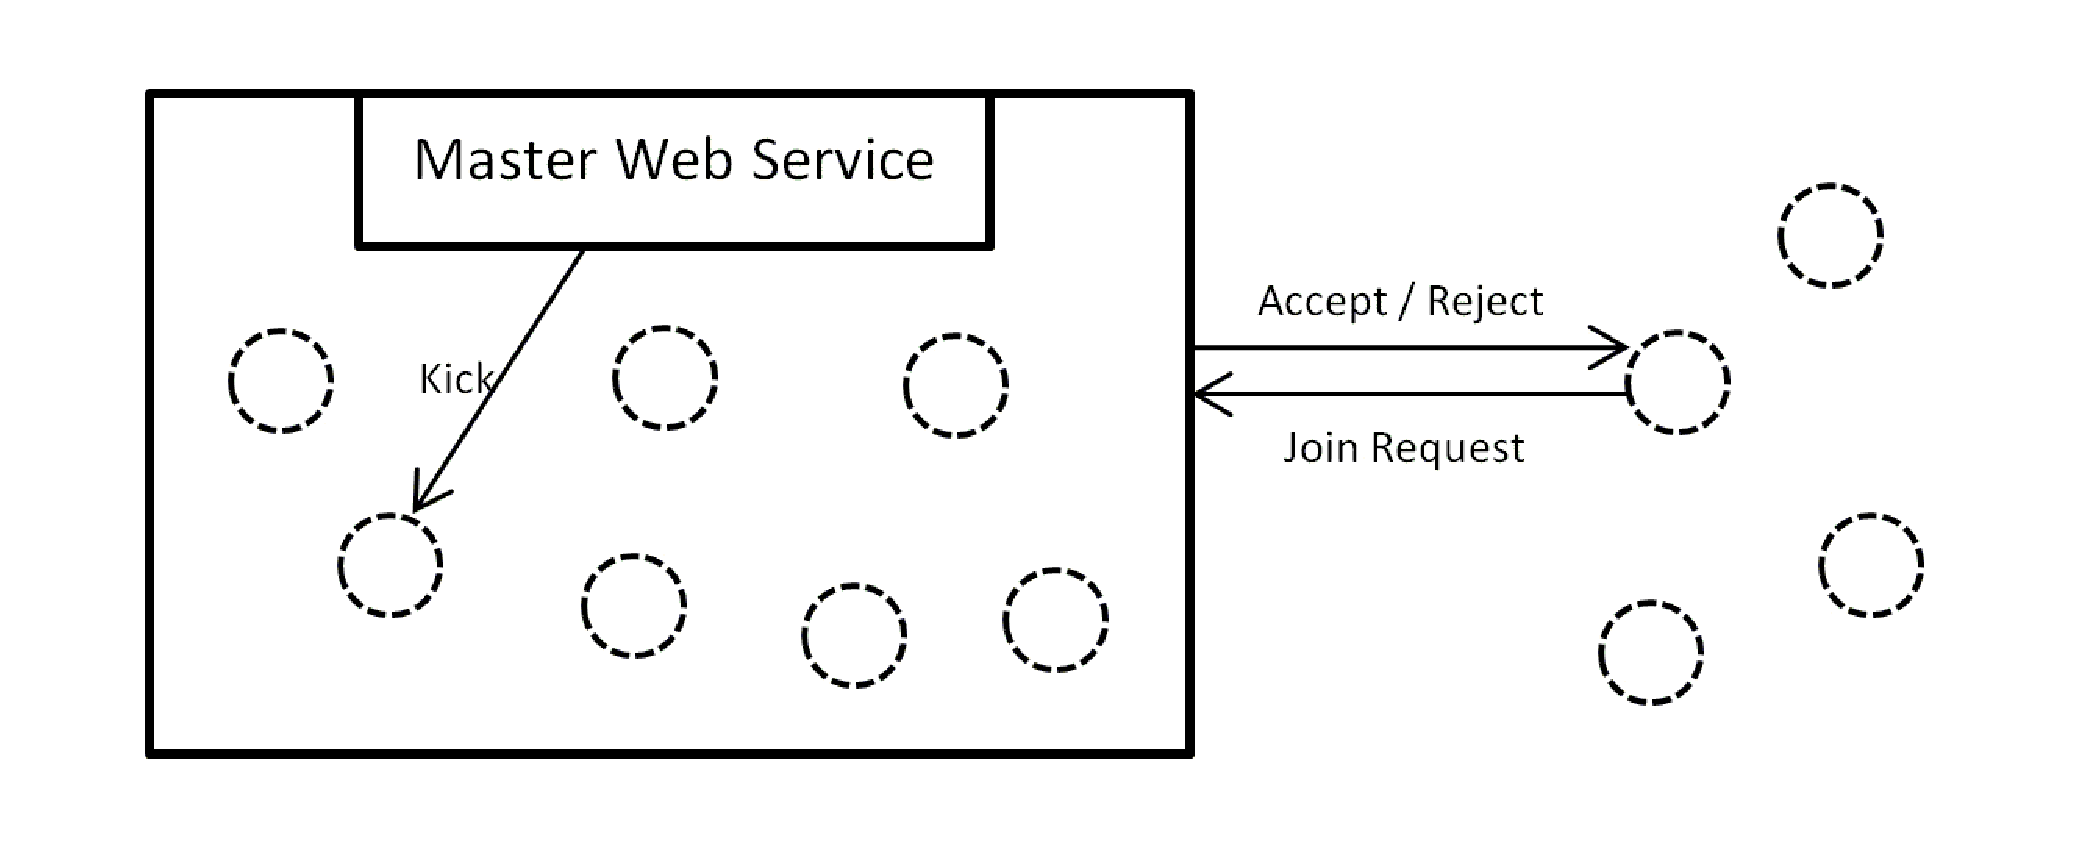
\includegraphics[width=3in]{s1.eps}
\caption{Web Services and A Grand Community}
\label{fig_sim}
\end{figure}

The membership decision is made based on throughput and QoS of the requested web service. The goal is to have quality web services in community so the community stays stable and no other web services would have incentives to deviate and join ``other'' coalitions. Therefore, we it check the core membership of the coalition of all current community members and the new web service. Our algorithm uses the Shapley value distribution method as described in equation \ref{eq:shapley} to distribute gain of $v(C)$ among all members and then checks if Shapley value payoff vector for this community having characteristic function $v(C)$ is Core stable or not. In Shapley value payoff vector, the payoff for each web service i, is calculated based on their contribution $v(C \cup {i}) - v(C)$ and then averaging over the possible different permutations in which the coalition can be formed, this is why Shapley value distribution is fair. It is proven in convex games the Shapley value lies in the core \cite{DBLP:conf/ijcai/GrecoMPS11, myerson1991game}. Therefore if the Core is non-empty, the Shapley payoff vector is a member of Core.
% so in our algorithm we check the core membership of this payoff vector. 

\emph{Proposition: } The folowwing statement is equivalent with convex condition of equation \ref{eq:convex}; 
\begin{equation}\label{eq:convex_snow}
v(S \cup \left\{i\right\}) - v(S) \leq v (T \cup \left\{i\right\}) - v(T), \forall S \subseteq T \subseteq N \backslash \left\{i\right\}, \forall i \in N; 
\end{equation}

\emph{Proof: } 

\begin{gather*}\label{convexsnowproof}
v(S \cup \left\{i\right\}) - v(S) \leq v (T \cup \left\{i\right\}) - v(T)
\\
\rightarrow v(S \cup \left\{i\right\}) + v(T) \leq v (T \cup \left\{i\right\}) + v(S)
\end{gather*}

We know $T \subseteq N - \left\{i\right\}$, therefore:

\begin{equation*}
(S \cup \left\{i\right\}) \cap T = T \cup S
\end{equation*}

and we have $S \subseteq T$, therefor:

\begin{equation*}
(S \cup \left\{i\right\}) \cap T = S
\end{equation*}

With a variable chnage of S we have:

\begin{gather*}
v(S \cup \left\{i\right\}) + v(T) \leq v (T \cup \left\{i\right\}) + v(S)
\\
\rightarrow v(S \cup \left\{i\right\}) + v(T) \leq v((S \cup \left\{i\right\}) \cup T) + v((S \cup \left\{i\right\}) \cap T)
\\
\rightarrow v(S^\prime) + V(T) \leq v(S^\prime) + v(S^\prime \cap T)
\end{gather*}

This means in order to keep the characteristic function convex, new agents should have more marginal contribution as coalition size grows.

Our algorithm works as follows. We have an established community with a master and some (slave) web services already residing in community. Now we have a request from a web service to join our community. The ideal solution in our method would be analyzing the core or $\epsilon-core$ stability of group having this new member. However the normal core membership algorithms are intractable. We exploit the equation \ref{eq:convex_snow} to check convexity of our characteristic function game having the new member. In that equation we set T to be our community members (C) before having the new web service. We set ${i}$ the new web service, and then verify the equation for S, setting $ S = T / W $ where $W$ is all 1-member subset of set C. We can relax the equation a bit by adding a constant epsilon to left side of equation. We call this method \emph{Depth-1 Convex-Checker} algorithm. If the equation is true for all $W$ we let the member join our community, since he will contribute good enough to make our new community stable. The run time complexity of this algorithm is O(n) which is huge reduction from $O(2^n)$ checking all possible subsets of N. In our second method, we use the same algorithm however this time we set W to be all possible subsets of size two and one of C. We call this method \emph{Depth-2 Convex-Checker} and its run time complexity is $O(n^2)$. It is possible to develop an anytime algorithm by continuing verifying this condition against all subsets of size 3 to N, and stop whenever we are interrupted.

\subsection {Web Services and Many Communities}

In this scenario we consider multiple communities owned by multiple master web services which provide independent request pools. Like first scenario master web services form coalitions with web services. We use coalition structure formation methods to partition web services into non-empty disjoint coalition structures. As mentioned in section \ref{sec:coalition} these algorithms \cite{DBLP:conf/ijcai/GrecoMPS11, DBLP:conf/ijcai/RahwanMJ11} try to solve two fundamental problems of what coalitions to form, and how will the members of these coalitions distribute their total gain to make these coalition structures stable. 

\begin{figure}[!t]
\centering
\includegraphics[width=3in]{s2.eps}
\caption{Web Services and Many Communities}
\label{fig_sim}
\end{figure}

The valuation function $v(C)$ for this scenario is same as \emph{one grand community} scenario, however in order to prevent master web services joining same community we set $v(C) = 0$, where C has two or more master web services as members. 

One of the properties of coalition structure formation algorithms in our scenario is that they partition web services with low throughput rate usually join coalitions with less request rate. Since the characteristic function $v(C)$ and  the fair payoff vector of Shapley value is proportional to web services' contribution, the web services with small contribution will get paid much less in communities having web services with high throughput. On the other hand, according to valuation function $v(C)$ web services with high throughput will not contribute well to communities with low amount of user requests. The strong web services are much more likely to deviate weak coalitions, joining a stronger coalition, making the initial coalition unstable.

In coalition-formation games, formation of the coalitions is the most important aspect of in the game. These solutions focus on maximizing social welfare. For any coalition structure $\pi$, let $v_{cs}(\pi)$ denote the total worth $\sum_{C \in \pi}{v(C)}$ which we call it social welfare. The problems in this area deal with finding the maximum value for social welfare over all the possible coalition structures $\pi$. There are $centralized$ algorithms for this end, however these approaches are generally NP-complete. The reason is that number of all possible partitions of a set $N$ grows exponentially with the number of players in $n$, and the centralized algorithms need to iterate through all these partitions. 
%These algorithms \cite{DBLP:conf/ijcai/GrecoMPS11, DBLP:conf/ijcai/RahwanMJ11, RePEc:wpa:wuwpga:0110001} are centralized algorithms, where all the complexity. However these algorithms are more intractable than Core stable solutions and practical with some constraints in practice\cite{RePEc:wpa:wuwpga:0110001}. 
In our application, we prefer not having a centralized decision maker dictating all web services their decisions. Becuase of this plus the complexity issues we would prefer a distributed algorithm where each community master can be a decision maker. The aim is to find low complexity and distributed algorithms for forming coalitions\cite{DBLP:journals/igtr/AptW09,Dieckmann02dynamiccoalition,ray2007game}. The distributed merge-and-split algorithm in \cite{DBLP:journals/igtr/AptW09} suits our application very well. It keeps splitting and merging coalitions where it is preferred by all players inside those coalitions. 
This merge-and-split algorithm is designed to be adoptable for different problems. It two functions to be specified, first a preference relation or comparison relation for comparing two collections of different coalition partitions of same players and second function is to assess the stability condition of a partition. Having two partition sets of a subset of our players, namely $P = {P_1,...,P_k}$ and $Q = {Q_1,...N_l}$ one example would be to use the social welfare comarison $\sum^k_{i=1}v(P_i) > \sum^k_{i=1}v(N_l)$. For our scenario we used $Pareto order$ comparison which is an individual-value order appropriate for our self-interest agents (web services). In Pareto order, an allocation or partition $P$ is preferred over another $Q$ if at least one player gets more payoff in new allocation without other players getting hurt, or other players at least same payoff. ($p_i \geq q_i$ with at least one element $p_i > q_i$). As new web services are discovered and get ready to join communities, this algorithm keeps merging and splitting partitions based on the preference or comparison function provides and will stop as the partitions satisfy the stability condition or no further merging and splitting is found satisfying the comparison function. More details of this algorithm and analyses of generic solutions on coalition formation games are described in \cite{DBLP:journals/igtr/AptW09}.

\subsection {Web Services collaborating independently}

In this scenario, we do not consider pre-defined communities and master web services. Here web services are interested in forming coalitions to perform better and share benefits. We do not consider concept of master web services providing requests for others, each web service comes with its own request load which in this scenario we call it \emph{market share}. Therefore coalitions will form is web services working together can perform and gain more than working alone individually. The worth or value of coalitions of web services is different in this setting, average the QoS metrics of web service, multiply it by a weight where the importance or weigth of each metric is dependent on type of users and requests web services are dealing with. For each web service we multiply this by web service's market share $(MarketShare_{ws})$ and the summation would be the characteristic or valuation of independent web service coalitions.

\begin{equation*}
v(C) = \sum_{ws}{\sum_{m=metrics}{\sum_{ws}{QoS^m_{ws} \times CC{m} \times ms_{ws}} \times w_{metric} } }
\end{equation*} 

$C_{coef}$ is \emph{Collabrative Coefficient} for each QoS metric, it determines how web services providing that QoS metric individually will be effected in a coalition environment. If it is more than 1, is means they increase performance by working together and they are \emph{super additive}, otherwise it depicts they would perform better in linear sense if they worked alone. Since there are no master web services, we assume they either dynamically vote for one, or collaborate and agree on decisions and distribute task in round robin or fair fashion. Like ``Web Services and Many Communities'' scenario, both core coalition structure analysis and social welfare analysis are applicable in this scenario.

\begin{figure}[!t]
\centering
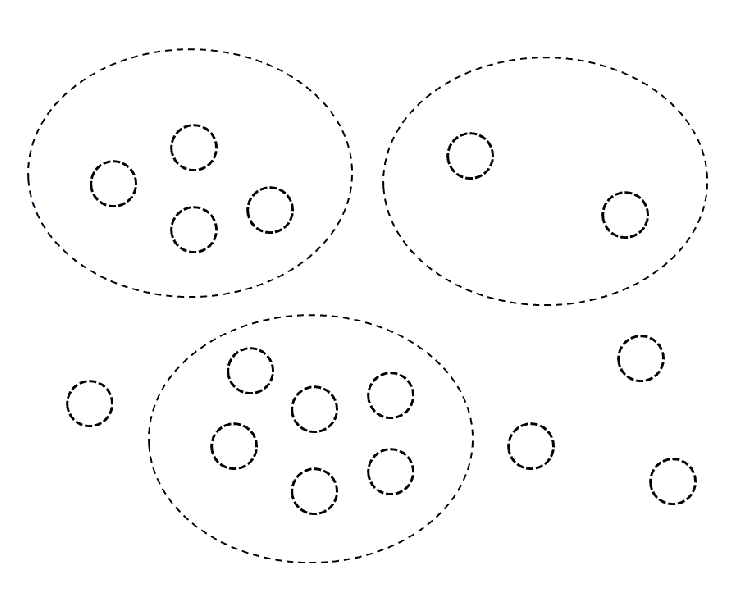
\includegraphics[width=3in]{s3.eps}
\caption{Web Services collaborating independently}
\label{fig_sim}
\end{figure}

\section{Experimental Results}

In this section, we discuss the experiments we performed for our scenarios to validate applicability and performance of our proposed methods in realistic environments. We created a pool of web services and populated most of their QoS parameters from a real world web service dataset \cite{DBLP:conf/smc/Al-MasriM09a}. We programmed the simulations using Java and executed the simulations on a Intel Xeon X3450 machine with 4GBs of memory. For other parameters we used normal distribution with parameters that make most sense in real world examples.

We first analyze the most important performance result our communities should perform, quality and quantity of tasks successfully performed by our communities. This is the most important criteria for user satisfaction. We initiate the community with few web services, then let rejecting and accepting of random web services go for a while, after that we start task distribution for the communities and let them allocate tasks for web services. Then we measure the average output performance of tasks in communities following different methods. 

\begin{figure}[!t]
\centering
%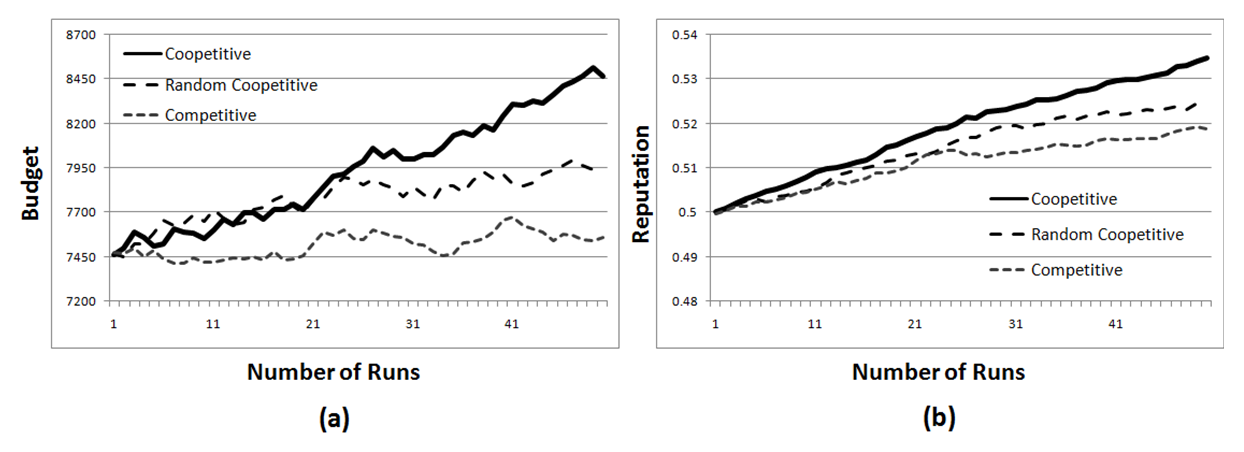
\includegraphics[scale=0.6]{graph1Final+.eps}
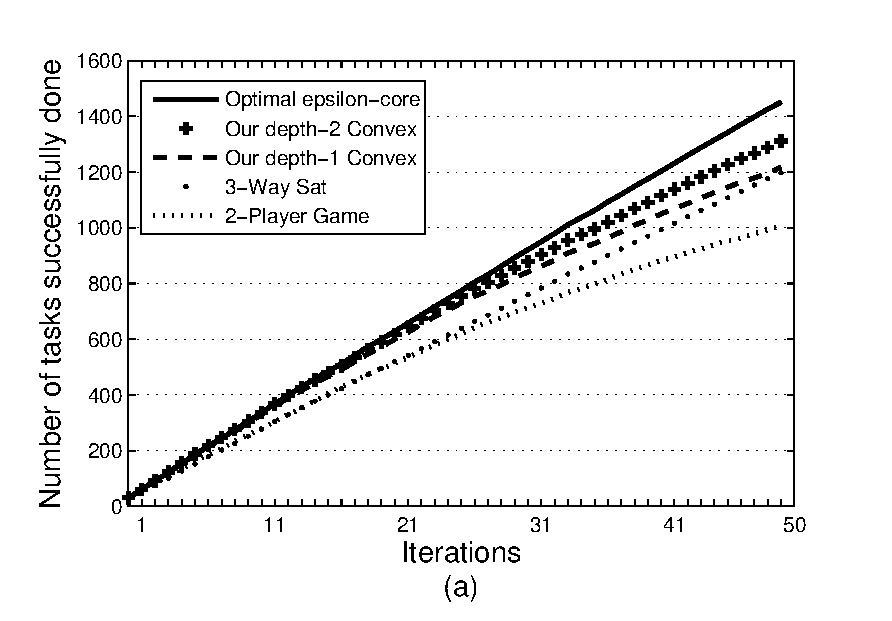
\includegraphics[scale=0.61]{task_done_opt.eps}
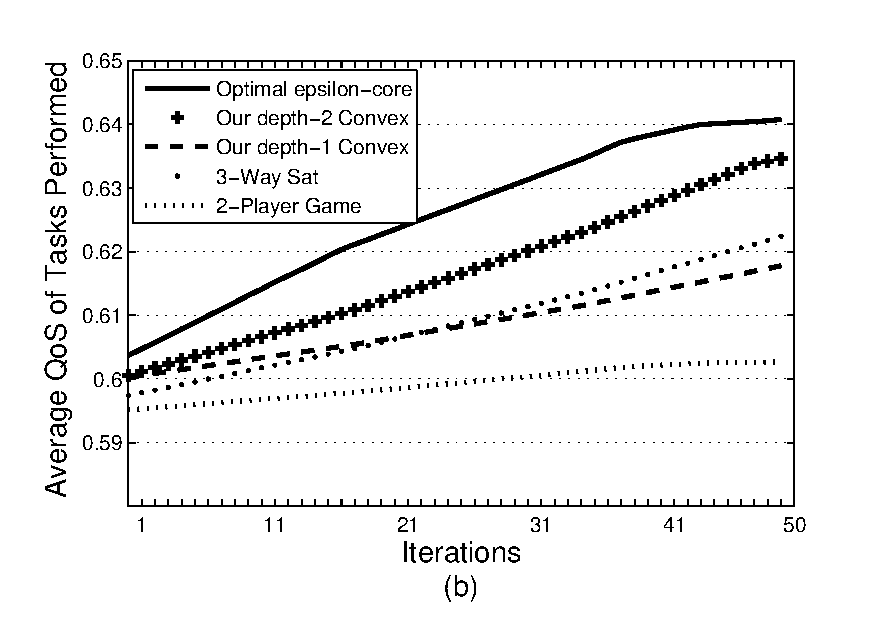
\includegraphics[scale=0.61]{task_qos_opt.eps}
\caption{Part (a): Cumulative number of tasks succesfully done. Part
(b): Average QoS of tasks performed.} \label{performanceall}
\end{figure}

Figure \ref{performanceall} depicts the results of simulation of optimal $\epsilon-Core$ with 10\% of total community value deviation allowed (one grand community with many web services), \emph{Depth-1 Convex-Checker}, \emph{Depth-2 Convex-Checker}, 3-Way Satisfactory\cite{DBLP:conf/IEEEscc/LimTMB12} and \emph{2 Player Non-Cooperative} methods. The the \emph{optimal $\epsilon$-core} method we capped the coalition size to 23 web services, since anything more than that would require analysis with time complexity of $O(2^22)$ which would made that impractical to run in our simulations. In other methods there were no cap on size of the community and we had communities of size 60 web services at some points. The results show depth-2 and 1 convex checker methods are performing well compared to other methods and all not far from optimal.


\begin{figure}[!t]
\centering
%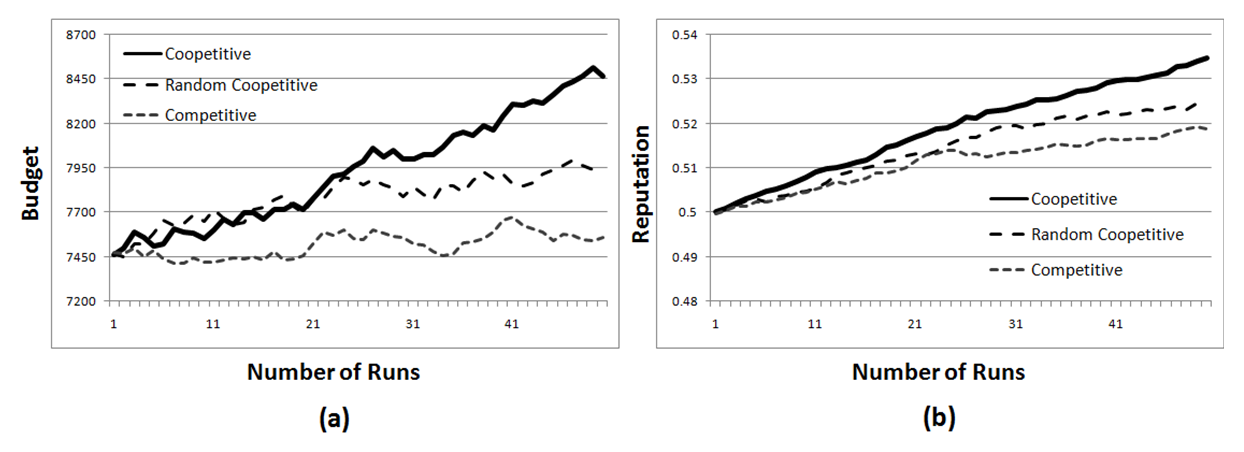
\includegraphics[scale=0.6]{graph1Final+.eps}
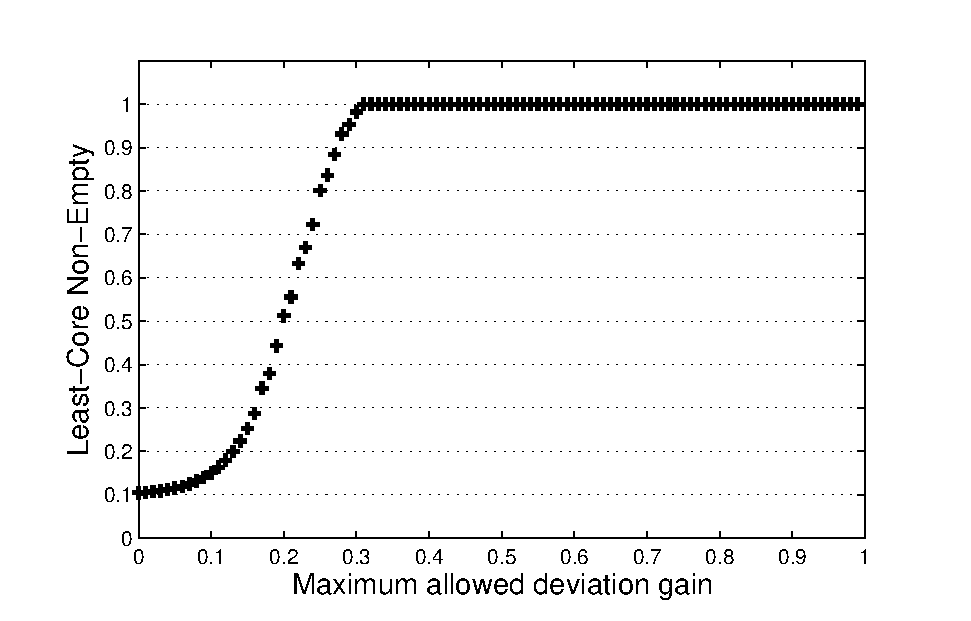
\includegraphics[scale=0.6]{least_core.eps}
\caption{Smallest value of $\epsilon$ such that the $\epsilon-core$ is non-empty} \label{f_leastcore}
\end{figure}

As mentioned in section \ref{s:epsilon}, core assumes no coalition of players can gain anything by deviating which is a fairly strong requirement, that is why the notion of $\epsilon-Core$ was introduced. Least-Core $e(G)$ of a game $G$, is the minimum amount of $\epsilon$ in which the core is not empty. We evaluated the least-core value using our valuation function and our set of web services. We pick random number of web services from our data set and form random coalitions consisting of 3 to 25 web services. We choose 25 as maximum number of members in our grand coalition since it is computationally very complex for bigger coalitions to compute least-core. We set $\epsilon$ to a ratio of total payoff of coalition v(C) from 0 to 1. The results in figure \ref{f_leastcore} show, almost in 10\% of random web service coalitions have non-empty core solution and least-core solution is always non-empty letting agents gain only 30\% more by deviating. 

\begin{figure}[!t]
\centering
%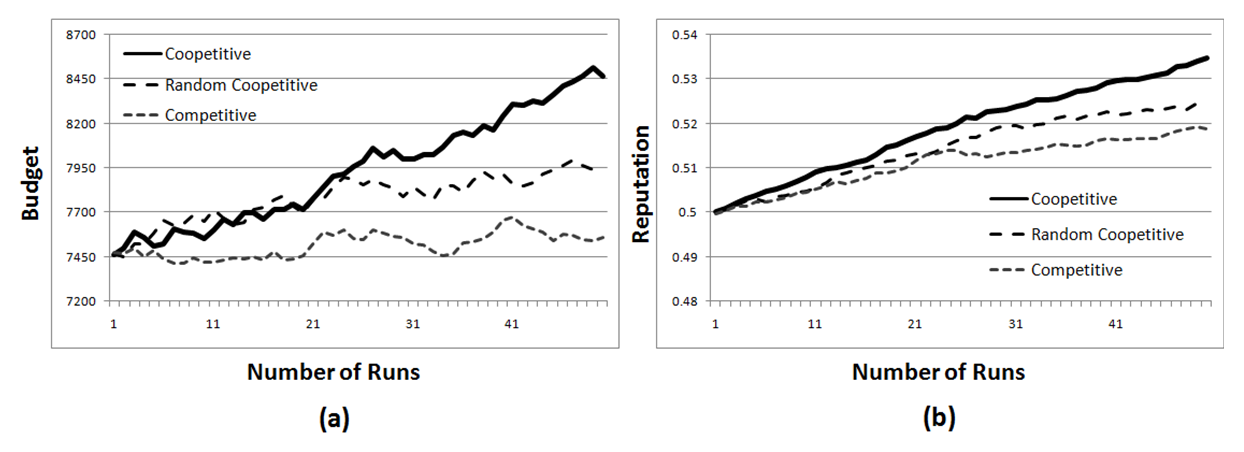
\includegraphics[scale=0.6]{graph1Final+.eps}
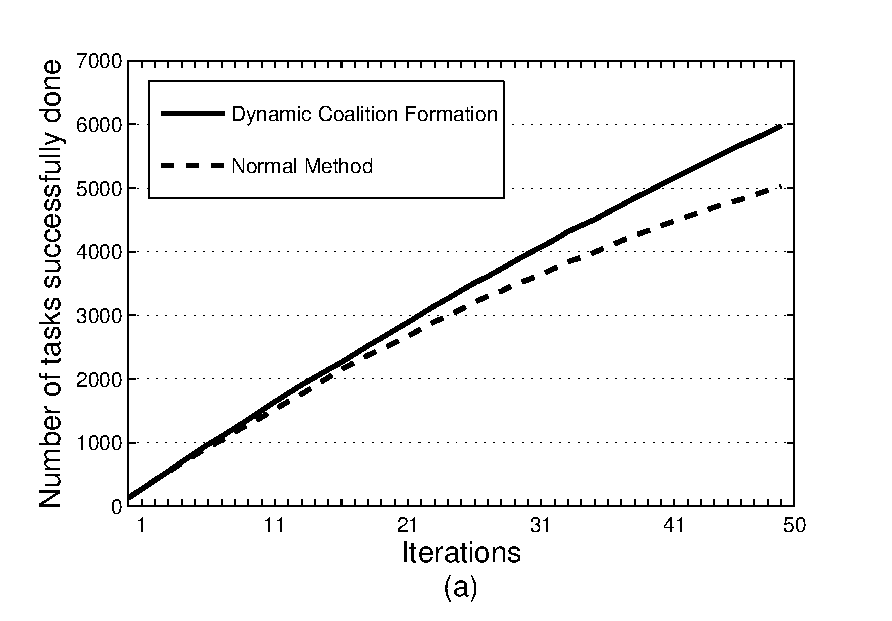
\includegraphics[scale=0.61]{s2_task_done.eps}
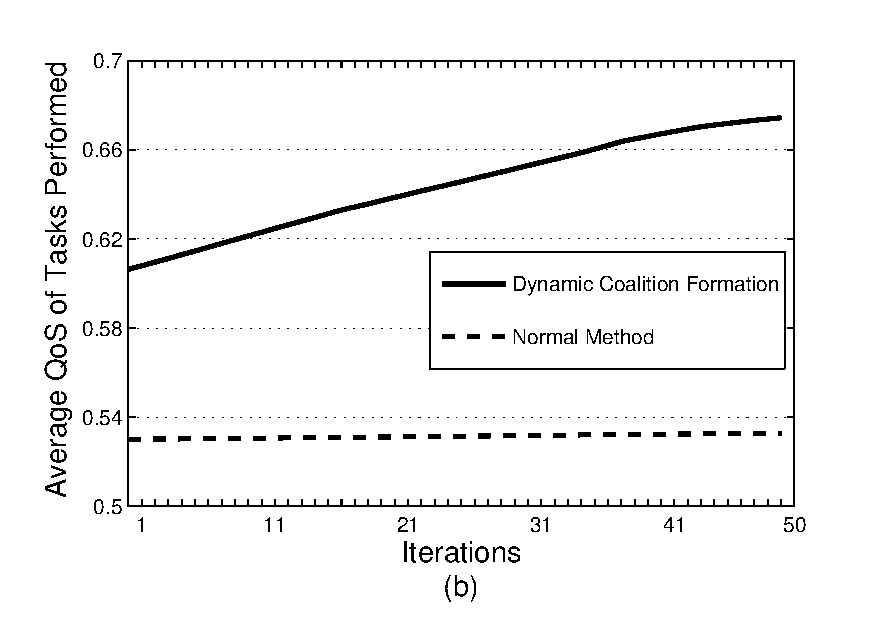
\includegraphics[scale=0.61]{s2_task_qos.eps}
\caption{Part (a): Cumulative number of tasks succesfully done. Part
(b): Average QoS of tasks performed.} \label{performancemany}
\end{figure}

In figure \ref{performancemany} we compare our \emph{Web Services and many Communities} scenario with a method which ignores QoS parameters and forms coalitions and allow web services to join only if they have enough requests for them in other words web services can join a community when request rate is less that throughput of all web services inside community ignoring QoS parameters. We name this method \emph{Normal method} and use it as our benchmark for our QoS aware coalition formation process. As results illustrate clearly, our QoS aware method, forms better coalitions of web services improving performance and satisfaction for both web service and coalitions. 

% An example of a floating figure using the graphicx package.
% Note that \label must occur AFTER (or within) \caption.
% For figures, \caption should occur after the \includegraphics.
% Note that IEEEtran v1.7 and later has special internal code that
% is designed to preserve the operation of \label within \caption
% even when the captionsoff option is in effect. However, because
% of issues like this, it may be the safest practice to put all your
% \label just after \caption rather than within \caption{}.
%
% Reminder: the "draftcls" or "draftclsnofoot", not "draft", class
% option should be used if it is desired that the figures are to be
% displayed while in draft mode.
%
%\begin{figure}[!t]
%\centering
%\includegraphics[width=2.5in]{myfigure}
% where an .eps filename suffix will be assumed under latex, 
% and a .pdf suffix will be assumed for pdflatex; or what has been declared
% via \DeclareGraphicsExtensions.
%\caption{Simulation Results}
%\label{fig_sim}
%\end{figure}

% Note that IEEE typically puts floats only at the top, even when this
% results in a large percentage of a column being occupied by floats.


% An example of a double column floating figure using two subfigures.
% (The subfig.sty package must be loaded for this to work.)
% The subfigure \label commands are set within each subfloat command, the
% \label for the overall figure must come after \caption.
% \hfil must be used as a separator to get equal spacing.
% The subfigure.sty package works much the same way, except \subfigure is
% used instead of \subfloat.
%
%\begin{figure*}[!t]
%\centerline{\subfloat[Case I]\includegraphics[width=2.5in]{subfigcase1}%
%\label{fig_first_case}}
%\hfil
%\subfloat[Case II]{\includegraphics[width=2.5in]{subfigcase2}%
%\label{fig_second_case}}}
%\caption{Simulation results}
%\label{fig_sim}
%\end{figure*}
%
% Note that often IEEE papers with subfigures do not employ subfigure
% captions (using the optional argument to \subfloat), but instead will
% reference/describe all of them (a), (b), etc., within the main caption.


% An example of a floating table. Note that, for IEEE style tables, the 
% \caption command should come BEFORE the table. Table text will default to
% \footnotesize as IEEE normally uses this smaller font for tables.
% The \label must come after \caption as always.
%
%\begin{table}[!t]
%% increase table row spacing, adjust to taste
%\renewcommand{\arraystretch}{1.3}
% if using array.sty, it might be a good idea to tweak the value of
% \extrarowheight as needed to properly center the text within the cells
%\caption{An Example of a Table}
%\label{table_example}
%\centering
%% Some packages, such as MDW tools, offer better commands for making tables
%% than the plain LaTeX2e tabular which is used here.
%\begin{tabular}{|c||c|}
%\hline
%One & Two\\
%\hline
%Three & Four\\
%\hline
%\end{tabular}
%\end{table}


% Note that IEEE does not put floats in the very first column - or typically
% anywhere on the first page for that matter. Also, in-text middle ("here")
% positioning is not used. Most IEEE journals/conferences use top floats
% exclusively. Note that, LaTeX2e, unlike IEEE journals/conferences, places
% footnotes above bottom floats. This can be corrected via the \fnbelowfloat
% command of the stfloats package.



\section{Conclusion}
The conclusion goes here. this is more of the conclusion

% conference papers do not normally have an appendix


% trigger a \newpage just before the given reference
% number - used to balance the columns on the last page
% adjust value as needed - may need to be readjusted if
% the document is modified later
%\IEEEtriggeratref{8}
% The "triggered" command can be changed if desired:
%\IEEEtriggercmd{\enlargethispage{-5in}}

% references section

% can use a bibliography generated by BibTeX as a .bbl file
% BibTeX documentation can be easily obtained at:
% http://www.ctan.org/tex-archive/biblio/bibtex/contrib/doc/
% The IEEEtran BibTeX style support page is at:
% http://www.michaelshell.org/tex/ieeetran/bibtex/
\bibliographystyle{IEEEtran}
\bibliography{bibi}
% argument is your BibTeX string definitions and bibliography database(s)
%\bibliography{IEEEabrv,../bib/paper}
%
% <OR> manually copy in the resultant .bbl file
% set second argument of \begin to the number of references
% (used to reserve space for the reference number labels box)

%\begin{thebibliography}{1}

%\bibitem{IEEEhowto:kopka}
%H.~Kopka and P.~W. Daly, \emph{A Guide to \LaTeX}, 3rd~ed.\hskip 1em plus
%  0.5em minus 0.4em\relax Harlow, England: Addison-Wesley, 1999.
%H.~Kopka and P.~W. Daly, \emph{A Guide to \LaTeX}, 3rd~ed.\hskip 1em plus
%  0.5em minus 0.4em\relax Harlow, England: Addison-Wesley, 1999.
%\end{thebibliography}




% that's all folks
\end{document}


